\documentclass{article}
\usepackage[margin=1.2in]{geometry}
\usepackage{enumitem}
\usepackage[table]{xcolor}
\usepackage{multirow}
\usepackage{tikz}
\usepackage{hyperref}
\pagenumbering{gobble} % turn off page numbers


\begin{document}

\section*{Clue 1: The Caesar Cipher}

Use your Caesar Cipher wheel to decipher the following sentence. 

The key is \textbf{K}.

\vspace{5mm}

\begin{tabular}{*{39}{@{\hskip3pt}c}}
X & S & M & O! &   & Q & O & D &   & D & R & O &  & X & O & H & D &   & M & V & E & O \\ 
\underline{\hspace{.5cm}} & \underline{\hspace{.5cm}} & \underline{\hspace{.5cm}} & \underline{\hspace{.5cm}}! & 
\hspace{.3cm} & 
\underline{\hspace{.5cm}} & \underline{\hspace{.5cm}} & \underline{\hspace{.5cm}} & 
\hspace{.3cm} & 
\underline{\hspace{.5cm}} & \underline{\hspace{.5cm}} & \underline{\hspace{.5cm}} & 
\hspace{.3cm} &
\underline{\hspace{.5cm}} &  \underline{\hspace{.5cm}} & \underline{\hspace{.5cm}} & \underline{\hspace{.5cm}} & 
\hspace{.3cm} &
\underline{\hspace{.5cm}} & \underline{\hspace{.5cm}} & \underline{\hspace{.5cm}} & \underline{\hspace{.5cm}} \\
P & B & Y & W &   & W & K & B & M & O & V & V & K. \\
\underline{\hspace{.5cm}} & \underline{\hspace{.5cm}} & \underline{\hspace{.5cm}} & \underline{\hspace{.5cm}} &
\hspace{.3cm} &
\underline{\hspace{.5cm}} & \underline{\hspace{.5cm}} & \underline{\hspace{.5cm}} & \underline{\hspace{.5cm}} &
\underline{\hspace{.5cm}} & \underline{\hspace{.5cm}} & \underline{\hspace{.5cm}} & \underline{\hspace{.5cm}}. \\
\end{tabular}



\paragraph{Bonus} How would you go about determining the key if you didn't already know its value? (Hint: ``the'' is the most common three-letter word in the English language.)

\newpage

\section*{Clue 2: Authentication}

In the last clue, we learned about \textit{encryption}, which lets us send a message to someone without anyone else being able to read it. 

Suppose you're sitting in class, writing notes on paper and passing them to your friend. The teacher notices and makes you two sit on opposite sides of the room. Now, this obviously won't stop you from passing notes, but now they have to go through 5 other people to get to the recipient. If any one of those 5 people was feeling rude, they could change the contents of your note.

\begin{minipage}{\textwidth}
\centering

\includegraphics[width=.6\textwidth]{tampered}
\end{minipage}

Now your friend can't tell what you wrote and what was changed by someone else. Our new goal is to find a way to check whether the text of the note you receive is the same as the text of the note that was sent. This is called \textit{authentication}.

To do this, we use a tool called a hash function. It takes in a message and outputs a short bit of gibberish. It's a one-way function, which means you can't go from gibberish to message. But, for any given message, it always outputs the same gibberish. 

\begin{minipage}{\textwidth}
\centering
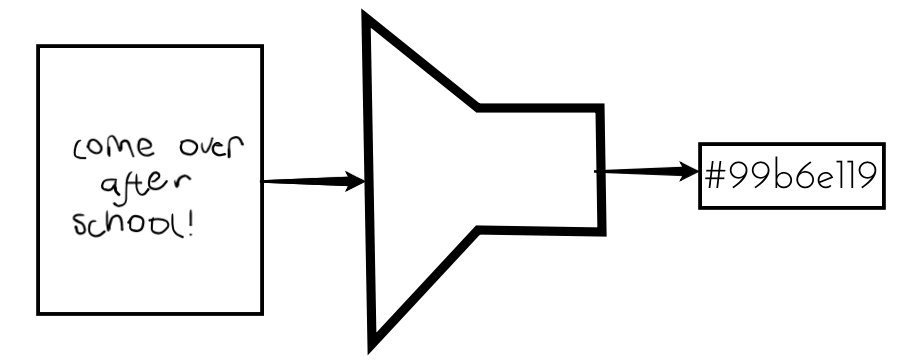
\includegraphics[width=.7\textwidth]{hash}
\end{minipage}

When you write a note, you'll calculate the hash of the message and write it at the end. When your friend receives the note, they'll calculate its hash and make sure it's the same as the one you provided. If they're different, she'll know someone tampered with the note.

Only one of these clues has a correct hash. You can check hashes at \url{http://www.seas.upenn.edu/~jpaykin/gems/auth.html}. Be sure to type the clues \textit{exactly}: even capitalization will change the hash (try comparing the hashes for ``wow'' and ``WOW''.) Identify the correct clue to get your next challenge!

\begin{enumerate}
  \item Get your next clue in Towne 100. \#c645be1c
  \item Get your next clue at your grandmother's house. \#3c6292ca
  \item Get your next clue from Achala. \#ac139d05
  \item Get your next clue from under your desk. \#bbee200f
\end{enumerate}

\newpage

\section*{Clue 3: What is a number, anyways?}

Did you know that computers only understand only 0s and 1s? Everything that you
see or hear on the computer---words, pictures, numbers, movies and even sound---is
stored using just those two numbers! But how? 

Numbers can be represented in all sorts of ways. We usually think of numbers in
the \emph{decimal} or \emph{base-ten} representation, like $3$, $49$, or $205$.
It's called base-ten because there are ten digits:
\begin{center}\begin{tabular}{cccccccccc}
    0 & 1 & 2 & 3 & 4 & 5 & 6 & 7 & 8 & 9
\end{tabular}\end{center}
When you have numbers larger than nine, each extra digit is multiplied by a
power of ten:
\[
    49 = 4\times10 + 9\times1 \qquad\textrm{and}\qquad 
    205 = 2\times100 + 0\times10 + 5\times1
\]
The \emph{binary} representation is called base-two, because it uses only
two digits: 0 and~1. 

To understand binary, take a look at the five cards in front of you, which are
powers of two:

\begin{minipage}{\textwidth}
\centering
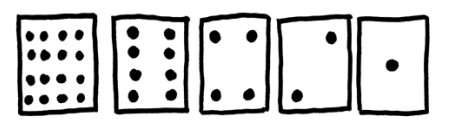
\includegraphics[width=.7\textwidth]{dots}
\end{minipage}
To represent a number, each card can either be turned up (displaying the dots)
or turned down (blank). Add up the number of dots shown to get the total number.
For example, to represent the number nine, you would use the following
combination of dots:

\begin{minipage}{\textwidth}
\centering
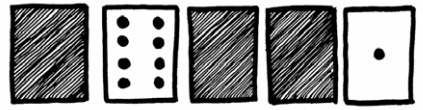
\includegraphics[width=.7\textwidth]{dots9}
\end{minipage}
Since we count the dots that are flipped upwards, but not the cards that are
flipped down, we can also think of that number as $0\times16 + 1\times8 +
0\times4 + 0\times2 + 1\times1$. In binary, this number is written $01001$:

\begin{minipage}{\textwidth}
\centering
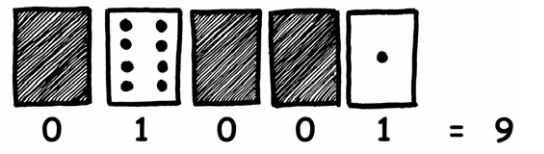
\includegraphics[width=.7\textwidth]{dots9'}
\end{minipage}

Practice using your own cards:
\begin{enumerate}
    \item What is the binary representation of the decimal number 4? % 00100
    \item What is the binary representation of the decimal number 12? % 01100
    \item What is the decimal representation of the binary number 10101? % 21
\end{enumerate}
There are 10 types of people in this world: those who understand binary, and
those who don't!


%TODO port \url{http://csunplugged.org/wp-content/uploads/2014/12/unplugged-01-binary_numbers.pdf} here.


To get your next clue, string together your answers to the questions above to
get a password (Hint: you will have 12 digits total), which you should enter in
the box at
\begin{center}
    \url{www.seas.upenn.edu/~jpaykin/gems/passwd.html}
\end{center}
Good luck!
  
\newpage


\section*{Clue 4: ENIAC}
ENIAC was one of the first programmable computers ever made. It was designed for use by the United States army and was used mainly to do calculations. The advent of computers meant that calculations that took hours or days to do by hand, only took minutes to solve automatically.

Do some research on ENIAC. To receive your next clue, go to the current location of ENIAC and report the names of the first six computer programmers for ENIAC.

TODO more questions?

\newpage

\section*{Clue 5: Designing an Algorithm}
Computers are pretty straightforward creatures: you tell them what to do, and they do it. If you tell it to do something unreasonable, it won't sanity-check you. It'll go ahead and do \textit{exactly} what you asked for.

The set of instructions you give a computer is called an \textit{algorithm}. For example, in Clue 1, you used the Caesar cipher algorithm to encrypt text like this:
\begin{enumerate}[noitemsep]
  \item Choose a letter as your key
  \item Write down the regular alphabet, starting with A.
  \item Underneath that, write down your secret alphabet, starting with the key.
  \item Write down the word you'd like to encrypt.
  \item For each letter in the word, find the corresponding secret letter and write it underneath the original letter.
  \item The letters you write down are the encrypted message.
\end{enumerate}

Today we'll try a different kind of algorithm. Describe how to create a butter and jelly sandwich. Write down the steps below. When you're satisfied with your algorithm, bring it to an instructor to check. Once your algorithm creates a standard sandwich, you will receive your next clue. Feel free to add more steps!

\paragraph{Sandwich Instructions:}
\begin{enumerate}
  \item
  \item
  \item
  \item
  \item
  \item
  \item
\end{enumerate}

\newpage

\section*{Clue 6: Picture perfect}
We've learned how to encrypt and authenticate a text-based message. However, in many cases we may wish to send a different type of data, like a picture. In order to use our existing encryption methods, we need to find a way to represent images using only text.

You may have seen a TV ad that brags about a number, like 1080i or 720p. That number refers to the number of pixels on the screen: a 1080 TV screen is actually made up of a giant grid of pixels, 1920 wide and 1080 tall. Each pixel can be a single color at a given time, so more pixels means a higher-definition image.

What this also means is that we can define single moment on a TV screen by listing out the color of each pixel. This means we need two things: a unique way to reference each pixel, and a way to determine the color. We'll deal with black and white images today: if a pixel is  ``on'' then it's black, and if it's ``off,'' it's white. 

The problem that remains is how we're going to refer to each pixel. Let's look at a small example.

\begin{center}
\begin{tabular}{*{5}{|c}|}
\hline
 &  &  &  &  \\ \hline
 &  &  &  &  \\ \hline
 &  &  &  &  \\ \hline
\end{tabular}
\end{center}

Here we have a $3\times 5$ grid of pixels (a very tiny TV). There are a couple ways we could refer to this. We could just number the boxes.

\begin{center}
\begin{tabular}{*{5}{|c}|}
\hline
1 & 2 & 3 & 4 & 5 \\ \hline
6 & 7 & 8 & 9 & 10 \\ \hline
11 & 12 & 13 & 14 & 15 \\ \hline
\end{tabular}
\end{center}

If we want to color in the top box in the middle, we'd add a step to our algorithm:


\begin{minipage}[c]{.4\linewidth}
\center
turn on box 2
\end{minipage}
\begin{minipage}[c]{.2\linewidth} $\rightarrow$ \end{minipage}
\begin{minipage}[c]{.4\linewidth}
\center
\begin{tabular}{*{5}{|c}|}
\hline
 & \cellcolor{gray!25} & & & \\ \hline
 & & & & \\ \hline
 & & & & \\ \hline
\end{tabular}
\end{minipage}


But if we're going to get into massive grids the size of TV screens and larger, these numbers will get really large, really quickly. We need a more efficient way to label the boxes.

Since we're dealing with a rectangular grid, every box has both a row and a column. We could use the row and column to uniquely refer to the boxes, which decreases the size of the numbers we use to refer to elements, with a tradeoff of needing two numbers for each box. 

\begin{center}
\begin{tabular}{*{7}{c|}}
\multicolumn{1}{c}{} & \multicolumn{6}{c}{Columns} \\ 
\multicolumn{2}{c}{} & \multicolumn{1}{c}{1} & \multicolumn{1}{c}{2} & \multicolumn{1}{c}{3} & \multicolumn{1}{c}{4} & \multicolumn{1}{c}{5} 
\\ \cline{3-7}
\multirow{3}{*}{Rows} & 1 & & & & & \\ \cline{3-7}
                      & 2 & & & & & \\ \cline{3-7}
                      & 3 & & & & & \\ \cline{3-7}
\end{tabular}
\end{center}

% TODO get rid of this dumb vertical line

To color in the same box as before, we'd refer to it by its row and column: 

\begin{minipage}[c]{.4\linewidth}
\center
turn on box (1,2) 
\end{minipage}
\begin{minipage}[c]{.2\linewidth} $\rightarrow$ \end{minipage}
\begin{minipage}[c]{.4\linewidth}
\center
\begin{tabular}{*{5}{|c}|}
\hline
 & \cellcolor{gray!25} & & & \\ \hline
 & & & & \\ \hline
 & & & & \\ \hline
\end{tabular}
\end{minipage}

Your final clue is an image, but we've encoded it into text format. To complete the scavenger hunt, you'll need to convert it back to an image. Color in the given coordinates to finish!

\newpage

\begin{tabular}{|*{10}{l}|}
\hline
(1,1) & (1,2) & (1,3) & (1,5) & (1,6) & (1,7) & (1,8) & (1,9) & (1,11) & (1,12) \\
(1,13) & (2,1) & (2,2) & (2,3) & (2,4) & (2,10) & (2,11) & (2,12) & (2,13) & (3,1) \\
(3,2) & (3,12) & (3,13) & (4,2) & (4,12) & (5,1) & (5,13) & (6,1) & (6,3) &
(6,4) \\
(6,5) & (6,9) & (6,10) & (6,11) & (6,13) & (7,1) & (7,3) & (7,4) & (7,5) & (7,9) \\
(7,10) & (7,11) & (7,13) & (8,1) & (8,4) & (8,10) & (8,13) & (9,1) & (9,6) &
(9,7) \\
(9,8) & (9,13) & (10,2) & (10,12) & (11,2) & (11,12) & (12,3) & (12,4) & (12,10) & (12,11) \\
(13,5) & (13,6) & (13,7) & (13,8) & (13,9) & & & & & \\
\hline
\end{tabular}

\vspace{1cm}

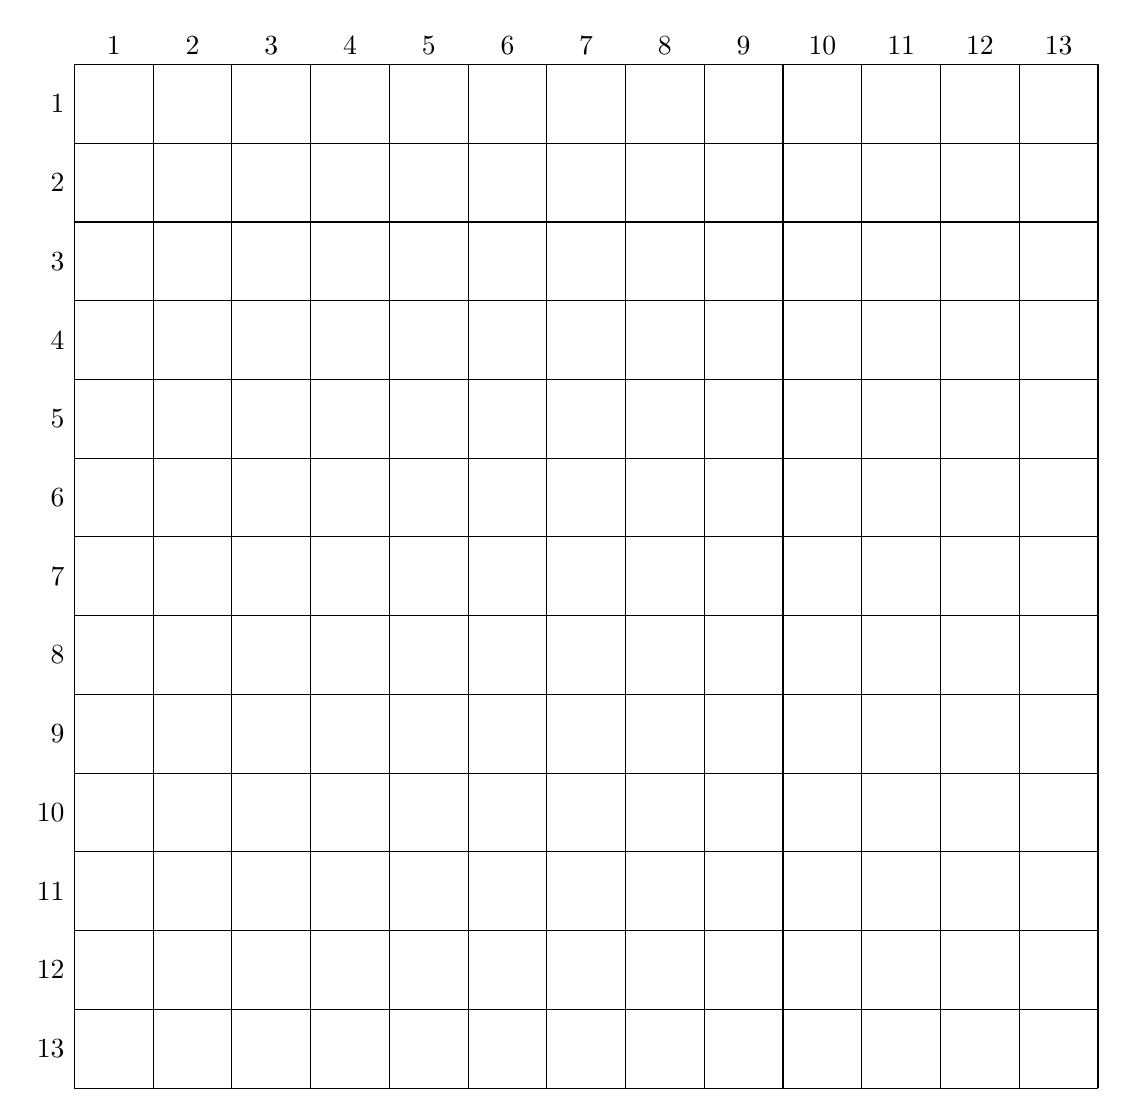
\begin{tikzpicture}
  \draw (0,0) grid (13,13);
  \foreach \x in {1,...,13}{
    \node[anchor=east] at (0, 13.5 -\x) {\x};
    \node[anchor=south] at (\x - 0.5,13) {\x};
  }
\end{tikzpicture}
\end{document}





%%% Local Variables:
%%% mode: latex
%%% TeX-master: t
%%% End:
